\section{\textbf{Count Down Latch}}
\subsection{Particular Case}
\par
The purpose of this experiment to our eyes is to demonstrate how monitor locks and conditions are used. Let us remember both concepts before going further.
\par
The concept of monitor consists on encapsulating three components: data, methods and synchronization mechanism. This allows to have our datastructures (or classes) take care of synchronization instead of overwhelming the user of the API with this task. \par
Now, the concept of \textit{conditions} comes into play because with them we can signal threads about an event. For example, instead of having threads spinning waiting for a value to become false, we can instead signal threads and let them know that they can now re-check for their locking condition.
\par
\subsection{Solution}
\par
The java interface for \textit{Lock} suggests two methods to implement the protocol drafter above. First, there is a method \textit{await()} which basically asks the thread wait till it is signaled about an event. The accompaning method \textit{signalAll} achieves this latter task.
\par
\subsection{Experiment Description}
\par
This experiment is a bit different from others showed before. The idea in this experiment is to show how the methods \textit{await()} and \textit{signalAll()} are combined in a working program. 
\par
So, the idea of the test is the following. Initially we have 8 threads. We start them as usual but we do not allow them to procced normally. Instead, we will ask them to wait for a signal. Internally, what we do is decrement a shared variable. When this variable becomes 0, the signal is triggered. Initially this signal is 1, meaning that we only need to decrement the variable once.
\par
After that, each thread will started and wait for the next signal. The variable that controlls this other signal is initially set to 8. Each thread will be in charge of decrementing this variable by one. Once it becomes 0, the second signal will be triggered announcing that our test must finish.
\par
These are the details of the system we used to run the experiments:
\begin{itemize}
\item Processor: Intel Core i5 @2.5 GHz. 2 Cores.
\item L2 Cache per Core: 256 KB
\item L3 Cache: 3 MB
\item System Memory: 16 GB
\end{itemize}
\subsection{Sample Results}
\par
For this test, we saw that in every try, it always passed.
\par
\begin{figure}[h]
  \centering
  \includegraphics[width=13cm]{CountDown00.png}
  \caption{Successful execution of the tests for Count Down latch}
  \label{fig:CountDown00}
\end{figure}
\par
\begin{figure}[h]
  \centering
  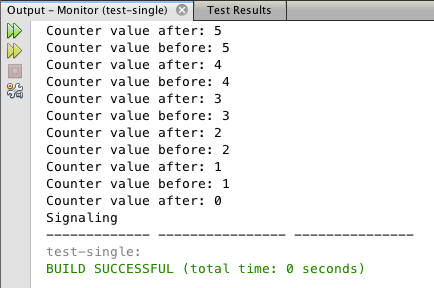
\includegraphics[width=8cm]{CountDown01.png}
  \caption{Successful execution of the tests  for Count Down latch}
  \label{fig:CountDown01}
\end{figure}
\par
\subsection{Interpretation}
This experiment showed us the way in which Monitors are used. We saw that we did not need to continously poll for a flag to acquire a lock. Instead, the monitor sent the threads a signal to indicate them that a particular condition has been met. In our particular test, these signals indicated: (1) that the threads can start; and (2) that the threads must stop.
